\chapter{Asking Billionaires How They Got Rich! (Beverly Hills)}

These notes follow the School of Hard Knocks interview on Beverly Hills, curated in this volume by LazyingArt LLC. The lecture is not a blackboard lecture in the ordinary sense; its mathematics is hidden inside revenue claims, starting conditions, payment order, market-size arithmetic, and financing structure. We therefore stay close to the order of the transcript and write down only those equations and relations that the spoken material genuinely motivates.

\section{Cold Open and Rodeo Drive Reset}

The lecture begins by spending surprise before it spends explanation. A teaser montage throws out a billionaire self-identification, a company sale, millionaire-at-seventeen language, large annual sales, and a dismissive line about schooling. We should not treat that opening as a stable ledger. Its function is to promise scale and tension.

\begin{remark}
The cold open is a splice of later claims. In these notes we use it only as an overture. The real argument begins when the host resets in Beverly Hills and frames Rodeo Drive as a field site for asking how wealth was built.
\end{remark}

That reset is important. We are no longer merely looking at luxury; we are being asked to extract mechanisms from it. The lecture therefore proceeds as a sequence of cases, each case offering a different local rule: starting below zero, listening before selling, surviving shocks, noticing detail, respecting market size, financing acquisition, and understanding how place affects price.

\section{Busboy to Boardroom: Starting Below Zero}

The first substantial case comes from hospitality. We move quickly from biography to arithmetic: busboy to boardroom, Diamond Resorts, Hilton, hotels in many countries, and then the shock of beginning not from zero but from a negative position. The transcript gives the essential starting condition as
\begin{equation}
W_0 = -\$20\,\text{million}, \qquad N_{\text{countries}} = 35.
\end{equation}
This is the first strong quantitative point of the lecture. Wealth here is not narrated as the simple accumulation of surplus from a comfortable baseline. It begins in deficit.

The same interview then gives two large valuation figures. Because the transcript is noisy, we record them cautiously:
\begin{equation}
V_{\text{eq}} \approx \$2.2\,\text{billion}, \qquad V_{\text{EV}} \approx \$3.3\,\text{billion}.
\end{equation}
The labels are uncertain, but the structure is clear enough: the speaker wants us to see the scale of the transformation from negative starting wealth to a company-valued enterprise.

The transition from biography to method comes through debt discipline. The speaker says that he never over-levered himself and that others were paid before he paid himself. The clean mathematical content is an ordering relation:
\begin{equation}
\text{Pay(partners)},\ \text{Pay(banks)} \prec \text{Pay(owner)}.
\end{equation}
This is not a legal waterfall; it is a moral and operational rule. Owner extraction is residual. The business must first remain trustworthy to those who fund it.

\subsection{Question \& Answer}

Question: why does the lecture make listening the real sales mechanism rather than persuasion alone?

Answer: because the lecture treats information as prior to pressure. The speaker compresses his sales doctrine into the single word \emph{listen}, and then immediately clarifies that customers, friends, and bankers reveal the pathway. We may therefore write
\begin{equation}
\mathrm{listen} \Rightarrow \text{pathway to sale}.
\end{equation}
The point is not passivity. Listening is the way we learn what counts as value to the counterparty. Only then does the second line make sense:
\begin{equation}
V_{\text{delivered}} \ge P_{\text{asked}}.
\end{equation}
If we do not know what the other side values, we do not know what must be delivered. The lecture's logic is therefore: listen first, price second.

\section{Negotiation, Banks, and Exogenous Shock}

The same interview widens from sales into negotiation and then further outward into the ecology of capital and crisis. Negotiation is first reduced to a blunt rule:
\begin{equation}
\mathrm{speak\ first\ in\ ripe\ deal} \Rightarrow \text{weaker bargaining position}.
\end{equation}
This should not be mistaken for a theorem of bargaining theory. It is a field rule: once the deal is ready, the first unnecessary utterance gives away informational advantage.

The lecture then makes an apparently strange move: it connects negotiation style to banking relationships. The speaker says he never negotiated hard with his banks; instead he made sure his banks made money with him. We should not universalize that claim, but the transcript is clear that, for this speaker, the lender relationship is a repeated game. The local aim is not minimal rate in one encounter, but continuity of support across many encounters.

From there the lecture makes a still larger move, from counterparties to exogenous shock. The stated example is the hotel business after 9/11:
\begin{equation}
R_{\text{hotel}} \to 0 \qquad \text{after the flight-stoppage shock.}
\end{equation}
This is one of the sharpest causal reductions in the chapter. Flights stop, guests vanish, the cash register goes to zero. Nothing in this account depends on product quality or salesmanship; it is pure exposure to a macro event.

\subsection{Question \& Answer}

Question: why does the lecture place silence in negotiation, generosity toward banks, and crisis survival inside one commercial worldview?

Answer: because in all three cases the lecture is thinking about endurance rather than momentary victory. The pattern is as follows.
\begin{enumerate}
\item In negotiation, we preserve informational advantage by not speaking too soon.
\item In financing, we preserve relational capital by making lenders and investors willing to stay in the game.
\item In crisis, we discover whether the system surrounding the business can absorb an external blow.
\end{enumerate}
The lecture's worldview is therefore not merely tactical. It is ecological. One must know how to act inside a network of customers, lenders, investors, and shocks.

This same widening continues in the human environment. The speaker warns against the ``bad zip code,'' meaning bad people, and against visible luxuries one cannot truly afford. We should read this as a non-equational but very important relation between social placement and financial outcome. The lecture is saying that business method is inseparable from the company one keeps.

\section{Listening at Operational Resolution: The Salon Case}

After the first recap, the lecture returns to the same doctrine from a more granular angle. The host generalizes listening into customer feedback, and the salon founder shows what that means at the operational level. The transcript gives a clean cluster of quantities:
\begin{equation}
S_{\text{salon}} = \$155\,\text{million}, \qquad E_{\text{operator}} = 50\%, \qquad C_{\text{raised}} \approx \$75\,\text{million}.
\end{equation}
The story begins with no money, a brother who had made some money at Yahoo, and a sweat-equity arrangement in which operating labor substitutes for cash contribution. Then the business grows large enough to raise substantial capital and eventually sell.

The host introduces a failure-rate heuristic:
\begin{equation}
p_{\text{fail},5\text{yr}} \approx \frac{8}{10}.
\end{equation}
We should keep this as a speaker-side estimate, not as an audited statistic. What matters for the lecture is not the exact number, but the reason that follows: most firms fail because they do not pay attention to the details that matter.

\subsection{Question \& Answer}

Question: why do tiny environmental details become business-killing variables?

Answer: because the lecture treats customer experience as an accumulation of small frictions and small reassurances. That logic can be written compactly as
\begin{equation}
\text{feedback ignored} \Rightarrow \text{fit deteriorates} \Rightarrow \text{customer exit}.
\end{equation}
The speaker then supplies the operational content of this chain: the bathroom is clean or not; the front desk has attitude or not; the chair scrapes loudly or not; the room feels cared for or not. None of these details looks grand in isolation. Together they produce the hidden state that customers feel before they can fully name it.

The section then broadens from customer fit to investor fit. The speaker says one must be careful who one gets into business with, because raising money from the wrong people creates a long-term mismatch in vision. The notes should preserve the lecture's metaphor here: capital is not just a check; it is a marriage. What matters is alignment on the future form of the business.

\section{The Interrupted Middle: Mentorship as Host Doctrine}

At this point the lecture deliberately interrupts itself. The School of Mentors segment is not another case study but the host's own institutional doctrine. The transcript gives the following scale claims:
\begin{equation}
N_{\text{millionaires interviewed}} > 1000, \qquad N_{\text{billionaires interviewed}} > 10,
\end{equation}
and also
\begin{equation}
F_{\text{followers}} \approx 10\,\text{million}, \qquad N_{\text{members}} \approx 2000.
\end{equation}
These numbers belong to the host's self-description, not to the interviewees' commercial method. Still, the interruption is structurally important. It tells us how the channel itself interprets the interviews: there is, according to the host, one shortcut to success, and that shortcut is mentorship.

For our purposes this section should remain short. It is a real beat in the lecture, but it is not the main source of the chapter's mathematical payload.

\section{Neil Patel: Reinvestment, ROI, TAM, and Acquisition}

The lecture now changes register. Earlier cases mixed story, aphorism, and rule of thumb. Neil Patel turns the discussion into cleaner arithmetic. The transcript gives us the following opening quantities:
\begin{equation}
t_{\text{entrepreneur}} = 23\,\text{years}, \qquad
R_{\text{firm}} \in \text{nine figures per year}, \qquad
D_{\text{owner}} \lesssim \$4\text{--}5\,\text{million per year}.
\end{equation}
The key distinction is between firm revenue and owner extraction. The point is not that the owner maximizes personal distribution, but that distributions are capped while retained earnings are reinvested into acquisitions, expansion, and hiring.

The marketing claim is similarly quantitative:
\begin{equation}
10^3 \le f_{\text{micro}} \le 10^5, \qquad
\mathrm{ROI}_{\text{micro}} > 30\%.
\end{equation}
Again, the transcript does not specify whether this is gross or net ROI, so we keep the statement exactly at the level the speaker gives it. The important point is that scale band matters: not celebrity-scale influence, but micro-influence with engaged communities.

\subsection{Question \& Answer}

Question: why can a good business still fail if the total addressable market is too small?

Answer: because even perfect execution cannot defeat an absolute ceiling. The lecture gives the standard arithmetic explicitly enough that we may formalize it.

\begin{definition}
If \(M\) denotes total addressable market and \(s\) denotes captured share, then the lecture's revenue relation is
\begin{equation}
R = sM.
\end{equation}
\end{definition}

The first example is the one stated directly by the speaker:
\begin{equation}
M=\$10\,\text{million}, \qquad s=1 \qquad \Rightarrow \qquad R=\$10\,\text{million}.
\end{equation}
This is the lecture's point in its simplest form: a tiny market stays tiny even when conquered completely.

To see the contrasting case numerically, we may take a representative market in the middle of the competitor range the speaker names:
\begin{align}
M &= \$16\,\text{billion}, \\
s &= 0.02, \\
R &= sM = 0.02 \times \$16\,\text{billion} = \$320\,\text{million}.
\end{align}
That number is not itself quoted in the transcript; it is a clean illustration of the arithmetic that the transcript is already using. A small share of a very large market can outrun total domination of a tiny one.

\begin{figure}[h]
\centering
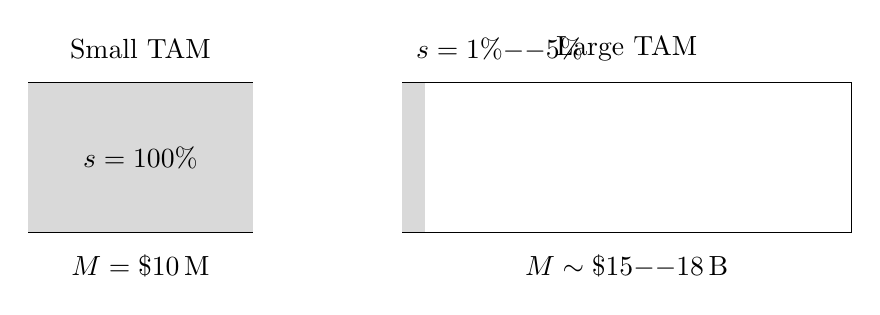
\begin{tikzpicture}[x=0.95cm,y=0.95cm]
\draw (0,0) rectangle (3,2);
\fill[black!15] (0,0) rectangle (3,2);
\node at (1.5,2.45) {Small TAM};
\node at (1.5,1.0) {$s=100\%$};
\node at (1.5,-0.45) {$M=\$10\,\mathrm{M}$};

\draw (5,0) rectangle (11,2);
\fill[black!15] (5,0) rectangle (5.3,2);
\node at (8,2.45) {Large TAM};
\node at (8,-0.45) {$M\sim \$15\text{--}18\,\mathrm{B}$};
\node at (6.3,2.45) {$s=1\%\text{--}5\%$};
\end{tikzpicture}
\end{figure}

The figure is only a transcript-led schematic, but it matches the lecture's logic exactly. Full ownership of the small rectangle still stays small. A narrow strip of the large rectangle may already be very large in dollars.

\paragraph{Worked example.}
The same section gives a compact derivation of early service-business growth through referrals. The transcript says that the first client paid
\begin{equation}
P_1 = \$5{,}000/\text{month},
\end{equation}
and that the work produced
\begin{equation}
\Delta R_{\text{client}} = \$25\,\text{million}.
\end{equation}
That performance generated three referrals, so the monthly run rate becomes
\begin{align}
N_{\text{referrals}} &= 3, \\
R_{\text{agency,monthly}} &= 4P_1 = 4\times \$5{,}000/\text{month} = \$20{,}000/\text{month}.
\end{align}
This is a very simple piece of arithmetic, but it is one of the lecture's cleanest compounding stories: good work produces referrals, and referrals scale recurring revenue.

\subsection{Question \& Answer}

Question: how can an operator start from zero and still buy a profitable business?

Answer: the lecture's answer is structural rather than fully numerical. One does not wait to accumulate the whole purchase price in cash. One layers financing:
\begin{equation}
\text{Acquisition financing} = \text{seller note} + \text{SBA-backed bank financing}.
\end{equation}
The retiring owner carries part of the note, the bank carries another part under SBA support, and the operating business is then improved through technology, rankings, reviews, and process discipline. The core idea is that the target's cash flow helps support the acquisition; the buyer's initial cash need not equal the full price.

\section{Transport, Place, and the Closing Rule}

The final interview is shorter and rougher, but it ends the lecture with a very portable pricing metaphor. The speaker argues that transport remains durable because goods must still move physically, and he reduces selling and negotiation to consistency and right-place-right-time presence. The real mathematical payoff, however, comes in the water example: the same bottle or glass of water changes price when moved from one place to another. The chapter can formalize the point as
\begin{equation}
P(w\mid L_1) \ne P(w\mid L_2),
\end{equation}
where \(w\) is the same good and \(L_1,L_2\) are distinct market contexts.

\subsection{Question \& Answer}

Question: why can the same good have a different price in a different place without changing its physical substance?

Answer: because price is not determined by substance alone. Place contributes convenience, scarcity, urgency, status, and the local demand structure. The speaker states this in street language rather than textbook language, but the logic is exact: valuation is conditional on context. We should therefore read the water example as a small theory of commercial placement.

The final rule of the lecture is mentorship. Here again the content is heuristic rather than formal, but it is clear enough to record:
\begin{equation}
\neg \text{mentor} \Rightarrow \text{directional drift}, \qquad
\text{mentor} + \text{observed bad moves} \Rightarrow \text{accelerated learning}.
\end{equation}
This closing line does not erase the earlier arithmetic. Rather, it gathers it. A mentor is valuable because he helps one see where the numbers, the relationships, and the hidden frictions actually sit.

\section{Summary}

The lecture begins by promising scale and ends by localizing scale into mechanisms. First, we are shown that business can begin from a negative starting condition,
\[
W_0=-\$20\,\text{million},
\]
and that discipline means paying others before oneself. Next, we are told that selling is not first a matter of pressure but of listening, so that value can be delivered against price. Then the same idea is pushed downward into operational detail: firms often fail because they do not hear what customers and employees are already telling them. Finally, the lecture reaches its most explicit arithmetic in the Patel section: revenue depends on market size,
\[
R=sM,
\]
reinvestment outruns extraction, and acquisition need not wait for full cash accumulation if financing is layered correctly.

What remains after the interviews is a compact set of rules. Begin even if the starting point is below zero. Keep counterparties whole. Listen before you speak. Respect the hidden force of detail. Prefer a large market to a perfect position in a tiny one. Understand that price is conditional on place. And treat mentorship, not as decoration, but as a device for seeing the structure of the game sooner.